\documentclass[conference]{IEEEtran}
\IEEEoverridecommandlockouts
% The preceding line is only needed to identify funding in the first footnote. If that is unneeded, please comment it out.
%Template version as of 6/27/2024


\usepackage{cite}
\usepackage{amsmath,amssymb,amsfonts}
%\usepackage{algorithmic} % Este ya no se usa, lo comento
\usepackage{graphicx}
\usepackage{textcomp}
\usepackage{xcolor}
\usepackage{bm}
\usepackage{lmodern}
\usepackage{fixmath}
\usepackage{comment}
\usepackage{algorithm}
\usepackage{algpseudocode}%
\usepackage{listings}%
\usepackage{manyfoot}%
\usepackage{booktabs}%


\usepackage{balance}
\definecolor{lightgray}{gray}{0.8}
\definecolor{darkgray}{gray}{0.4}

% Colors
\definecolor{matlabBlue}{rgb}{0.000,0.380,0.900} % vibrant blue for MATLAB/Simulink traces
\definecolor{springgreen4}{rgb}{0,0.55,0.27}
\definecolor{red4}{rgb}{0.55,0,0}
\definecolor{darkgreen}{rgb}{0,0.39,0}
\definecolor{darkred}{rgb}{0.55,0,0}
\definecolor{morado}{rgb}{.88,.50,.90}
\definecolor{azul}{rgb}{.5,.5,.98}
\definecolor{grisOscuro}{rgb}{.1,.1,.1}

% Tiny line-style swatches for figure captions (safe in moving arguments)
\DeclareRobustCommand{\legsolid}[1]{\textcolor{#1}{\rule[0.55ex]{1.6em}{0.45pt}}}
\DeclareRobustCommand{\legdotted}[1]{\textcolor{#1}{\makebox[1.6em][l]{\dotfill}}}






\def\BibTeX{{\rm B\kern-.05em{\sc i\kern-.025em b}\kern-.08em
    T\kern-.1667em\lower.7ex\hbox{E}\kern-.125emX}}
\begin{document}

\title{Neuromorphic Modeling and Control for a Coaxial Hexarotor UAV using Spiking Neural Networks}
\medskip

\begin{comment}
    

\author{
\IEEEauthorblockN{Anel Olivares C.}
\IEEEauthorblockA{\textit{Academic Area of Computing and Electronics} \\
\textit{Universidad Aut\'onoma del Estado de Hidalgo}\\
Mineral de la Reforma, M\'exico \\
anelolivarescruz@gmail.com}
\and
\IEEEauthorblockN{Gandhi Contreras}
\IEEEauthorblockA{\textit{Klipsch School of Electrical}\\ \textit{and Computing Engineering} \\
\textit{New Mexico State University}\\
Las Cruces, USA \\
gandhico@nmsu.edu}
\and
\IEEEauthorblockN{Victor J. Silva}
\IEEEauthorblockA{\textit{Aeronautical Engineering}\\\textit{Metropolitan Polytechnic}\\\textit{University of Hidalgo}\\
Tolcayuca, Mexico \\
223112167@upmh.edu.mx}
\and
\IEEEauthorblockN{Eduardo S. Espinoza}
\IEEEauthorblockA{\textit{Center for Research} \\
\textit{ and Advanced Studies of}\\\textit{
 the National Polytechnic Institute}\\
Mexico City, Mexico \\
eduardo.espinoza@cinvestav.mx}
\and
\IEEEauthorblockN{Juan M. Bustamante}
\IEEEauthorblockA{\textit{Center for Research} \\
\textit{and Advanced Studies of}\\\textit{the National Polytechnic Institute}\\
Mexico City, Mexico \\
juan.bustamantea@cinvestav.mx}
\and
\IEEEauthorblockN{Patricio Ordaz}
\IEEEauthorblockA{\textit{Academic Area of Computing and Electronics} \\
\textit{Universidad Aut\'onoma del Estado de Hidalgo}\\
Mineral de la Reforma, Mexico \\
jesus\_ordaz@uaeh.edu.mx}
}
\end{comment}
\maketitle


\begin{abstract}
Neuromorphic processors offer a promising path toward energy-efficient autonomous flight, but their practical adoption requires translating conventional flight-control algorithms into spiking neural networks (SNNs) while preserving closed-loop performance. This paper presents a neuromorphic flight-control architecture for a coaxial Hexarotor UAV based on the Neural Engineering Framework (NEF). Both the vehicle dynamics and the cascade flight controller are implemented as recurrent SNNs in the Nengo simulator. The Hexarotor dynamics are decomposed into altitude, longitudinal, lateral, and directional subsystems, while the controller employs PID regulation in the outer translational loops and PD regulation in the inner attitude loops. Performance is evaluated in a 60 s trajectory-tracking mission against an equivalent classic implementation of the same control architecture. The SNN-based controller achieves correlation coefficients exceeding 0.99 and sub-decimeter RMS position-tracking errors, demonstrating close agreement with the conventional controller. %The small residual discrepancies are consistent with finite-population neural coding effects inherent to SNN representations. 
\end{abstract}

\begin{IEEEkeywords}
UAV, Neural Engineering Framework, neuromorphic computing, spiking neural networks.
\end{IEEEkeywords}

\section{Introduction}\label{intro}

Unmanned Aerial Vehicles (UAVs) rely on autonomous navigation and flight-control algorithms that process information from multiple onboard sensors to perform guidance, stabilization, and trajectory tracking. As these algorithms become increasingly sophisticated, the computational requirements for real-time autonomy continue to grow, motivating the exploration of alternative computing paradigms beyond conventional von Neumann architectures.

Neuromorphic computing has emerged as a promising solution for energy-efficient real-time control. By integrating memory and computation within distributed spiking neural networks (SNNs), neuromorphic processors offer low power consumption, asynchronous computation, and inherent fault tolerance, making them attractive for autonomous aerial systems~\cite{rajendran_low-power_2019,bouvier_spiking_2019}. The Neural Engineering Framework (NEF)~\cite{eliasmith_how_2013,Eliasmith2011} provides a systematic methodology for representing nonlinear dynamical systems and controllers as SNNs, while the Nengo simulator enables their implementation and evaluation without requiring dedicated neuromorphic hardware.
Recent studies have demonstrated the feasibility of NEF-based SNN controllers for underactuated systems and quadrotor UAVs~\cite{OmarCCE,DiegoNICE,OmarACC,Olivares2025,olivares_self-tuning_2026}. Other works have validated neuromorphic control on dedicated hardware, such as Intel Loihi, for robotic manipulators~\cite{dewolf_neuromorphic_2023}. While previous studies have demonstrated the feasibility of SNN-based flight controllers on neuromorphic hardware for simplified UAV applications, including single-degree-of-freedom attitude stabilization~\cite{Stagsted2020,Vitale2020} and single-axis vertical landing based on optic-flow divergence~\cite{Dupeyroux2021}, these approaches are limited to reduced-order systems and focus primarily on the controller implementation. In such works, the vehicle dynamics are simulated or estimated using conventional numerical methods outside the neural framework. As a result, the development of a fully neuromorphic flight-control architecture, in which both the UAV dynamics and the cascade control system are represented within the Neural Engineering Framework (NEF), has received little attention, particularly for multirotor platforms beyond the conventional quadrotor. The proposed approach addresses this gap by providing a unified, modular, and scalable neural architecture in which both the vehicle dynamics and the flight controller are implemented as recurrent spiking neural networks, enabling a fully neuromorphic closed-loop representation from state evolution to control computation.

%To address this gap, this paper presents a fully neuromorphic modeling and control framework for a coaxial hexarotor UAV. The vehicle dynamics are decomposed into altitude, longitudinal, lateral, and directional subsystems, each represented as recurrent SNNs in the Nengo simulator. A classical cascade flight controller, comprising PID outer-loop position control and PD inner-loop attitude control, is implemented using the same neuromorphic framework and evaluated through trajectory-tracking simulations against an equivalent MATLAB/Simulink implementation. The results demonstrate that the proposed SNN-based realization accurately reproduces the closed-loop behavior of the conventional controller while establishing a scalable architecture for future neuromorphic flight-control systems.

The main contributions of this work are summarized as follows:
\begin{itemize}
    \item A neuromorphic modeling and control framework for a coaxial hexarotor UAV is developed by systematically mapping the reduced nonlinear vehicle dynamics and cascade flight controllers into recurrent spiking neural networks within the Neural Engineering Framework using the Nengo simulator.
    \item The proposed SNN-based controller is quantitatively validated through trajectory-tracking simulations against a conventional MATLAB/Simulink implementation employing PID controllers in the outer translational loops, and PD controllers in the inner attitude loops, demonstrating high agreement in closed-loop performance.
    \item A modular and scalable NEF-based architecture is established for implementing flight-control systems as interconnected spiking neural populations, providing a foundation for future deployment on neuromorphic hardware and the integration of more advanced neural control strategies.
\end{itemize}

The remainder of the manuscript is organized as follows.
Section~\ref{Modeling} presents the Newton--Euler-based mathematical
model of the hexarotor UAV and its corresponding spiking neural
network representation. Section~\ref{Control} describes the
conventional cascade control strategy employed for trajectory tracking
and the development of its neuromorphic counterpart.
Section~\ref{Simulations} reports the simulation results and provides a
comparative analysis of the conventional and neuromorphic control
implementations. Finally, Section~\ref{Conclusions} summarizes the main
findings and outlines directions for future research.

\section{Dynamic Modeling of the Coaxial Hexarotor}\label{Modeling}

In this section, the dynamics of the hexarotor depicted in Fig.~\ref{fig:hexarotor} are modeled and represented using SNNs. To facilitate neural encoding, analysis, and control design, the vehicle dynamics are decomposed into altitude, longitudinal, lateral, and directional subsystems. The translational and rotational equations of motion are first derived using the Newton–Euler formulation and subsequently mapped into an SNN-based representation implemented within the Nengo framework. The neural implementation is obtained through the third principle of the NEF, which enables the realization of dynamical systems using recurrently connected neural populations. This neuromorphic representation serves as the foundation for the modeling and control architecture developed in this study.

\begin{figure}[t]
    \centering
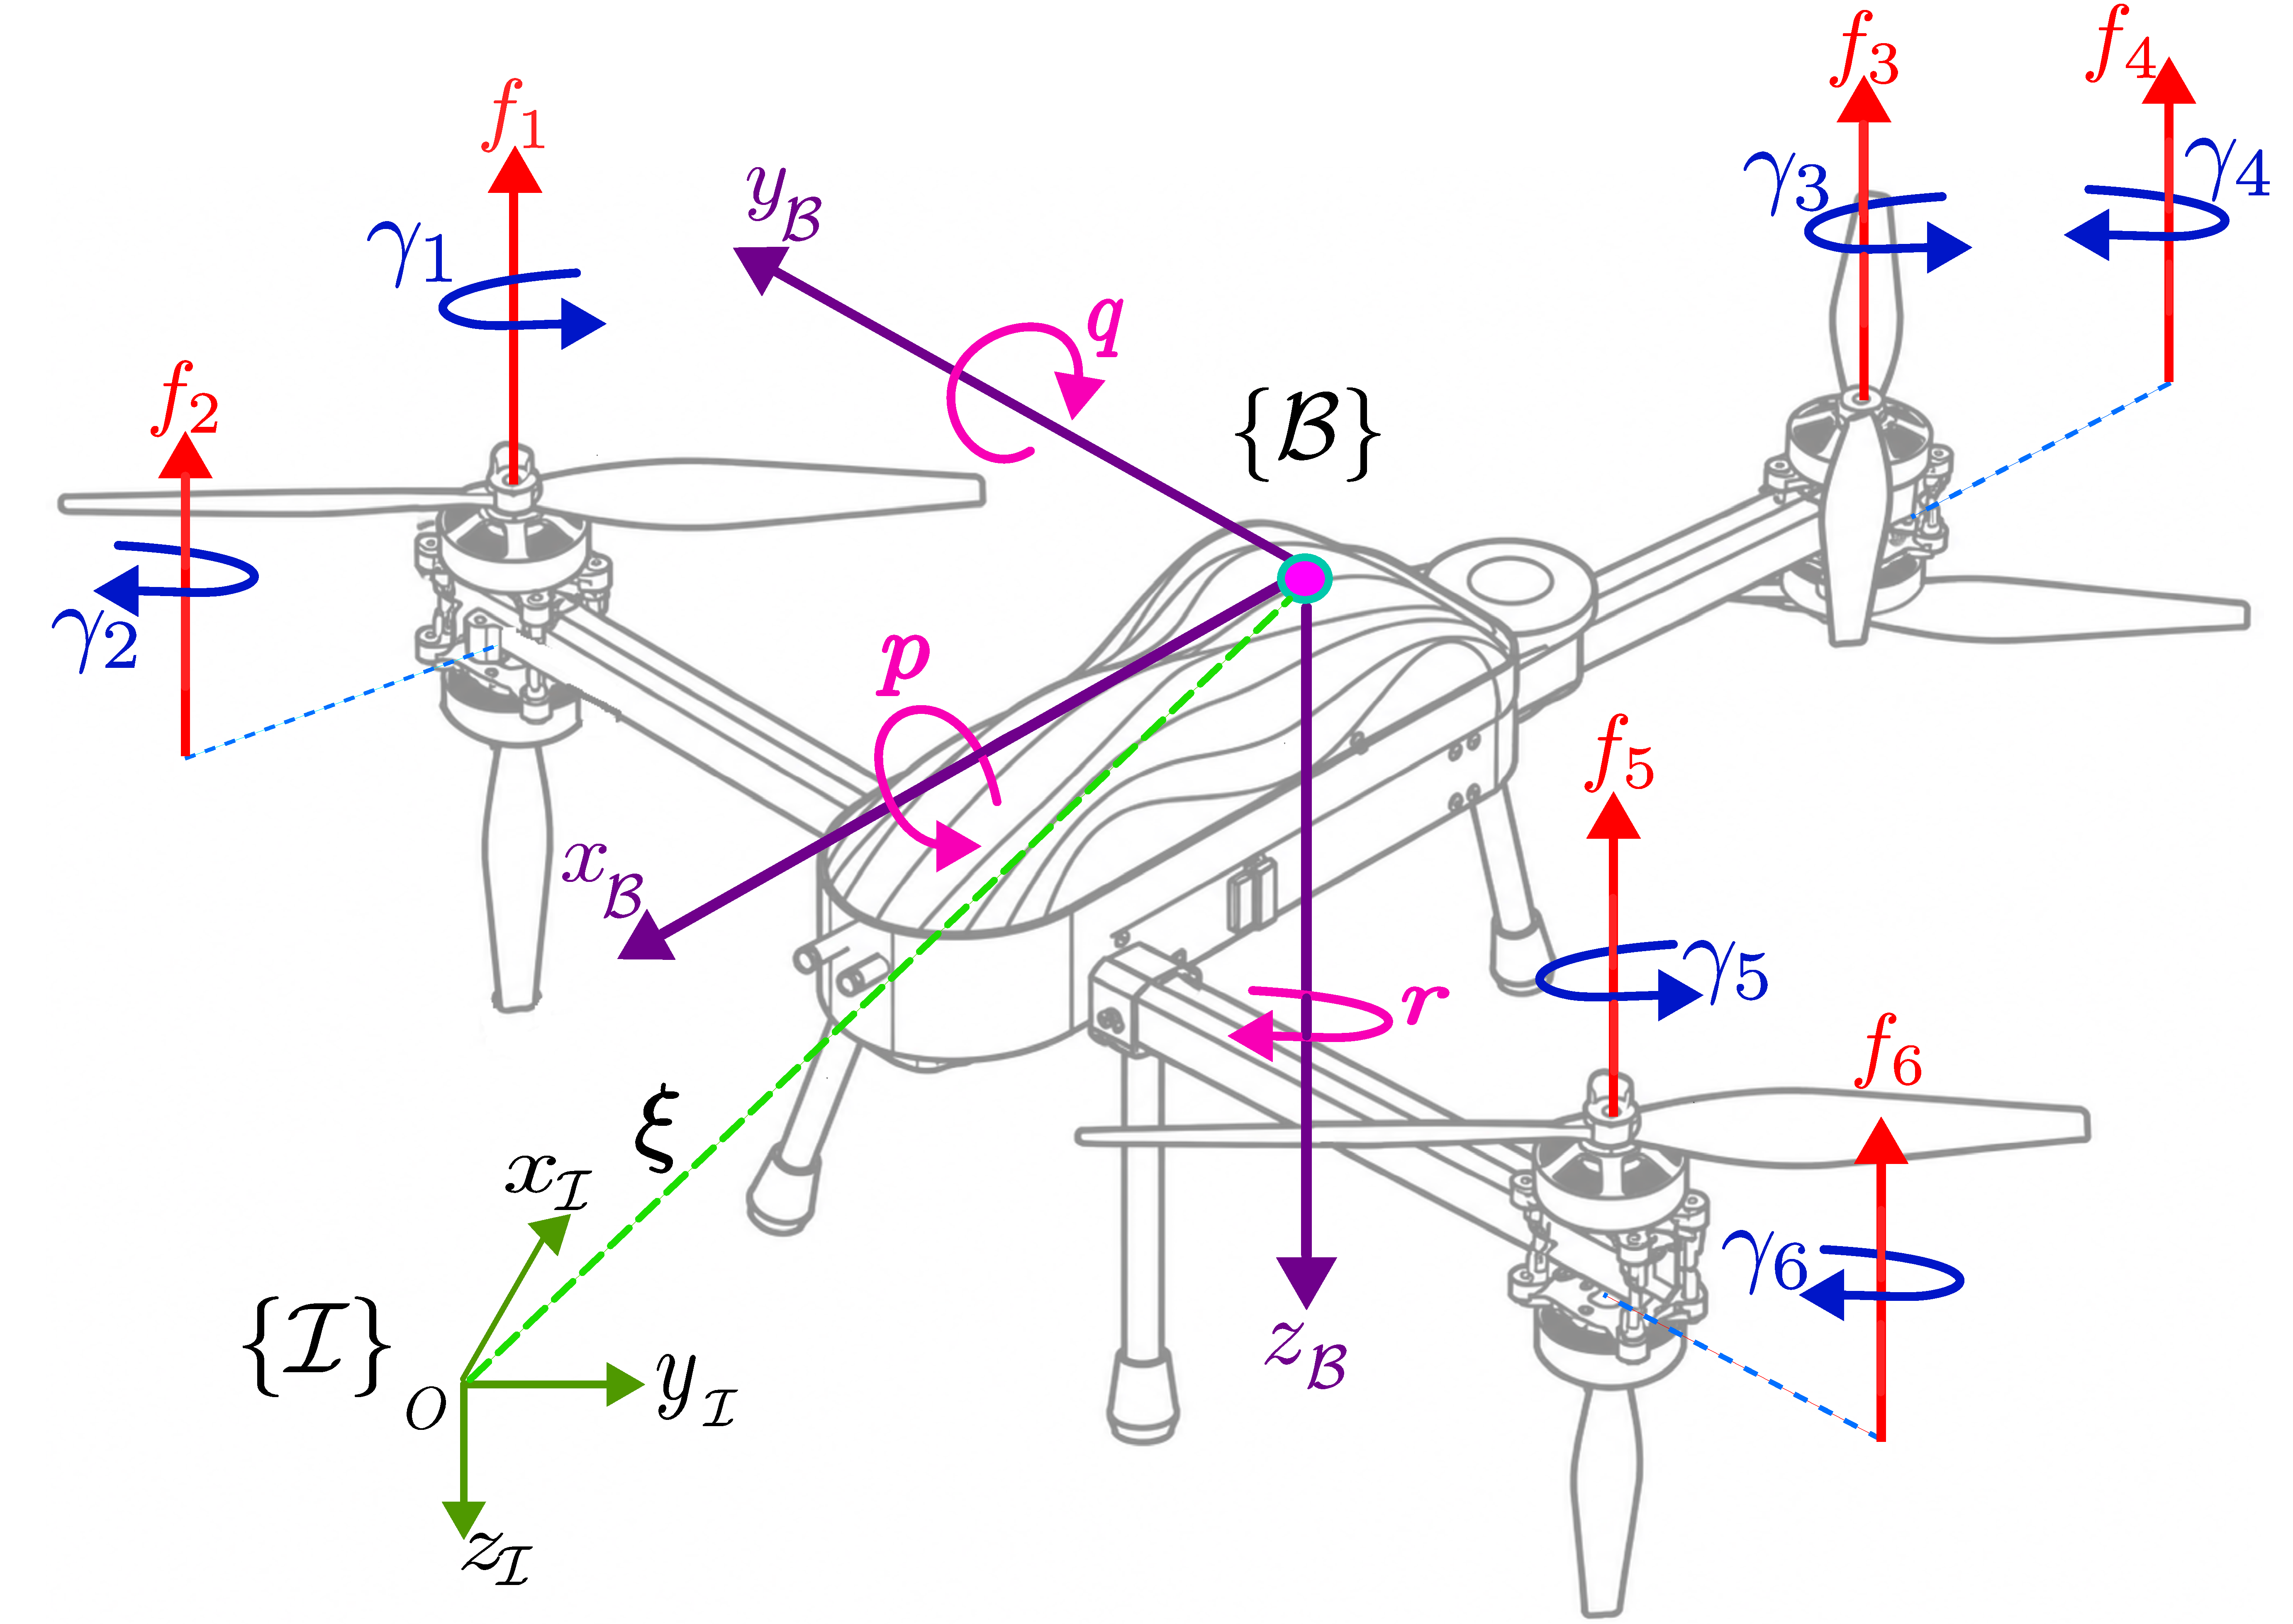
\includegraphics[width=\linewidth]{Figures/dinamica_hexa3.pdf}
    \caption{
    Coaxial hexarotor UAV: three arms with counter-rotating coaxial rotor pairs (T6 configuration), shown with the main airframe forces and the inertial $\{\mathcal{I}\}$ and body $\{\mathcal{B}\}$ NED frames. Its dynamics are stabilized by the proposed SNN-based cascade controllers.}
    \label{fig:hexarotor}
\end{figure}


\subsection{Newton-Euler Formulation}

For the hexarotor UAV shown in Fig.~\ref{fig:hexarotor}, let $\{\mathcal{I}\}$=$\{x_{\mathcal{I}},y_{\mathcal{I}},z_{\mathcal{I}}\}$ denote the inertial frame and $\{\mathcal{B}\}$=$\{x_{\mathcal{B}},y_{\mathcal{B}},z_{\mathcal{B}}\}$ the hexarotor body-fixed frame. The vehicle position expressed in the inertial frame is $\bm{\xi}=(x,y,z)^\top\in\mathbb{R}^{3}$ while its attitude is parameterized by the Euler angles $\bm{\eta}=(\psi,\theta,\phi)^\top\in\mathbb{R}^{3}$, corresponding to yaw, pitch and roll, respectively. The body angular velocity is $\bm{\Omega}=\left(p,q,r\right)^\top\in\mathbb{R}^{3}$, $m$ denotes the vehicle mass, and $\mathbb{I}\in \mathbb{R}^{3 \times 3}$ is the inertia matrix.


Using the Newton--Euler formulation, the rigid-body dynamics of the vehicle are given by: $\dot{\bm{\xi}} = \bm{V} $, $m\dot{\bm{V}} = \bm{R}\bm{F} $, $\dot{\bm{R}} = \bm{R}\hat{\bm{\Omega}}$, $\mathbb{I}\dot{\bm{\Omega}} = -\bm{\Omega}\times\mathbb{I}\bm{\Omega}+\bm{\Gamma}$, where
$\boldsymbol{V}\in\mathbb{R}^3$ is the translational velocity,
$\boldsymbol{F}\in\mathbb{R}^3$ is the total external force,
$\boldsymbol{\Gamma}\in\mathbb{R}^3$ is the total external moment,
$\hat{\boldsymbol{\Omega}}$ is the skew-symmetric matrix satisfying
$\hat{\boldsymbol{\Omega}}\mathbf{a}
=
\boldsymbol{\Omega}\times\mathbf{a}$ for any
$\mathbf{a}\in\mathbb{R}^3$, and
$\boldsymbol{R}\in SO(3)$ denotes the rotation matrix from
$\{\mathcal{B}\}$ to $\{\mathcal{I}\}$.


The total rotor thrust is defined as $u=\sum_{i=1}^{6} f_i$, acting along the body $z_{\mathcal{B}}$ axis. The control moments about the body axes are given by $\Gamma_\phi=l_1\,(f_1+f_2-f_5-f_6)$, $\Gamma_\theta=l_2\,(f_1+f_2+f_5+f_6)-l_3\,(f_3+f_4)$, and $\Gamma_\psi=(\gamma_1+\gamma_3+\gamma_5)-(\gamma_2+\gamma_4+\gamma_6)$. The thrust pairs $(f_1,f_2)$, $(f_3,f_4)$, and $(f_5,f_6)$ correspond to the three counter-rotating coaxial rotor pairs of the T6 configuration in Fig.~\ref{fig:hexarotor}. The constants $l_1$, $l_2$, and $l_3$ are the corresponding moment arms determined by the vehicle geometry, and $\gamma_i$ denotes the rotor drag torque (with sign given by the rotor spin direction). These virtual inputs $u$, $\Gamma_\phi$, $\Gamma_\theta$, and $\Gamma_\psi$ are the same variables commanded by the cascade controller in Section~\ref{Control}; in Section~\ref{Simulations}, rotor-level allocation is abstracted to isolate controller and neural-representation effects from mixing.

Neglecting aerodynamic effects and higher-order disturbances, the hexarotor dynamics are decomposed into altitude, longitudinal, lateral, and directional subsystems, which are sufficient for the controller design considered here. The reduced model assumes near-hover flight (small tilt angles and moderate speeds); large-angle maneuvers, strong wind, and rotor/actuator dynamics are not considered.

\medskip

\subsubsection{Altitude subsystem}
The vertical dynamics are described by
\begin{equation}\label{alt_dynamics}
\begin{aligned}
\ddot z &= -\frac{u }{m}\cos \theta \cos \phi + g 
\end{aligned}
\end{equation}

A feedback-linearizing controller for altitude regulation is chosen as 
%
\begin{equation}\label{eq:u}
    u= \frac{m}{\cos\theta \cos \phi}\left( g - \underbrace{\left(kp_z e_z+kd_z \dot e_z +ki_z\int e_zdt\right)}_{u_z}\right)
\end{equation}
%
where $e_z=z_d-z$, and $\dot e_z=\dot z_d-\dot z$, denoting the position and velocity tracking errors along the $z_\mathcal{I}$-axis, respectively.

\subsubsection{Longitudinal subsystem}
The longitudinal dynamics are
%
\begin{align}
\ddot x &= -\frac{u}{m} \left( \cos \phi \cos \psi \sin \theta + \sin \phi \sin \psi \right) \label{long_dynamics_x} \\
\ddot \theta &= \frac{\Gamma_\theta} {I_{yy}} \cos \phi -\frac{\Gamma_\psi}{I_{zz}} \sin \phi \label{long_dynamics_theta}
\end{align}

Substituting~\eqref{eq:u} into~\eqref{long_dynamics_x} and assuming small attitude angles $\sin(\alpha)\approx \alpha$, $\cos(\alpha)\approx 1$ and $\tan(\alpha) \approx \alpha$, for $\alpha=\{\theta,\phi,\psi\}$, the longitudinal dynamics reduce to:
%
\begin{align} \label{red_long_dynamics_x}
\ddot x = -g \tan \theta ,\quad  
\ddot \theta =  {\Gamma_\theta}/{I_{yy}} %\label{red_long_dynamics_theta}
\end{align}


\subsubsection{Lateral subsystem}
The lateral dynamics are
%
\begin{align}
\ddot y &= -\frac{u}{m} \left(\cos \phi \sin \theta \sin \psi - \cos \psi \sin \phi \right) \label{lat_dynamics_y}\\
\ddot \phi &=\frac{\Gamma_\phi}{I_{xx}} + \frac{\Gamma_\theta}{I_{yy}} \sin \phi \tan \theta  + \frac{\Gamma_\psi}{I_{zz}}  \tan \theta \cos \phi \label{lat_dynamics_phi}
\end{align}      

Applying the altitude control law and the small-angle approximations yields
%
\begin{align}\label{red_lat_dynamics_y}
\ddot y = g {\tan \phi}/{\cos \theta}, \quad
\ddot \phi = {\Gamma_\phi}/{I_{xx}} %\label{red_lat_dynamics_phi}
\end{align}

\subsubsection{Directional subsystem}
The yaw dynamics are given by
\begin{equation}\label{dir_dynamics}
\begin{aligned}
\ddot \psi &= \frac{\Gamma_\theta \sin \phi}{I_{yy}\cos \theta}   +  \frac{\Gamma_\psi \cos \phi}{I_{zz}\cos \theta}. \end{aligned}
\end{equation}

Under the small-angle assumption, the directional subsystem reduces to
%
\begin{equation}\label{red_dir_dynamics}
\ddot{\psi}
=
{\Gamma_\psi}/{I_{zz}}.
\end{equation}
%


\subsection{Neural Representation in Nengo}\label{FG_subsystems}
%
Within the NEF, nonlinear dynamical systems can be implemented as recurrent SNNs. As illustrated in Fig.~\ref{fig:NLS_population}, the recurrent connection of a spiking population implements the neural function $F'(\chi)$, which encodes the state dynamics, while the input connection implements $G'(\upsilon)$, which encodes the external inputs. Here, $\chi(t)$ denotes the system state, $\upsilon(t)$ the input vector, and $h(t)=\frac{1}{\tau}e^{-t/\tau}$ is the first-order synaptic filter describing the postsynaptic current generated by incoming spikes, with $\tau$ the synaptic time constant.
%
\begin{figure}[h]
    \centering
    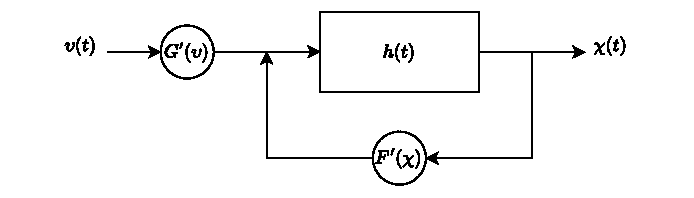
\includegraphics[width=\linewidth]{Figures/NLS_population.pdf}
    \caption{Neural representation of a nonlinear dynamical system using a recurrent spiking neural population.}
    \label{fig:NLS_population}
\end{figure}

The dynamics implemented by the recurrent neural population are given by the convolution of the synaptic filter with the neural functions. Let $W(t)=F'(\chi(t))+G'(\upsilon(t))$, then 
\begin{equation}
{\chi(t)} = h(t) * W(t)
\end{equation}
where $(*)$ denotes the convolution operator.

Applying the Laplace transform yields
%
\begin{equation}
s\chi(s) = \frac{1}{\tau}\bigl[W(s) - \chi(s)\bigr]
\end{equation}

Taking the inverse Laplace transform and substituting $W(t)$ gives the neural state equation
%
\begin{equation}\label{eq:NLS_n}
\dot \chi = \frac{1}{\tau}\bigl[F'(\chi)- \chi + G'(\upsilon)\bigr]
\end{equation}

Consider a nonlinear system described in state-space form as
%
\begin{equation}\label{eq:NLS}
    \dot \chi =F(\chi)+G(\upsilon),
\end{equation}
%
equating~\eqref{eq:NLS} and \eqref{eq:NLS_n} leads to the neural functions required to implement the dynamics in the recurrent neural population,
%
\begin{equation}\label{eq:NEF_map}
F'(\chi)= \tau F(\chi) + \chi; \quad G'(\upsilon) = \tau G(\upsilon).
\end{equation}

Each reduced subsystem
of~\eqref{alt_dynamics}--\eqref{red_dir_dynamics} is a double
integrator in its own coordinate. Defining the subsystem state
$\chi=[\zeta,\dot{\zeta}]^\top$ for
$\zeta\in\{z,x,\theta,y,\phi,\psi\}$, the dynamics take the form
$\dot\chi_1=\chi_2$, $\dot\chi_2=\upsilon_\zeta$, so that
$F(\chi)=(\chi_2,\,0)^\top$ and
$G(\upsilon_\zeta)=(0,\,\upsilon_\zeta)^\top$. Substituting
into~\eqref{eq:NEF_map} yields the common neural representation
\begin{equation}\label{eq:FG_generic}
F'_\zeta(\chi)=
\begin{bmatrix} \chi_1+\tau\chi_2\\ \chi_2 \end{bmatrix};
\qquad
G'_\zeta(\upsilon_\zeta)=\tau
\begin{bmatrix} 0\\ \upsilon_\zeta \end{bmatrix}.
\end{equation}
%%%%%%%%%%%%%%%%%%%%%%%%%%%%%%%%%%%%%%%%%%
\begin{figure*}[!ht]%t
    \centering
    \includegraphics[width=\linewidth]{Comrob_Hexa2026/Figures/Quadri_Victor_combination_PID_R2025a_CE_v3.drawio.pdf}
    \caption{Classical cascaded controller implementation used as the MATLAB/Simulink baseline. The outer position loops generate the translational control laws $u_x$, $u_y$, and $u_z$, while the inner loops generate the attitude control laws $u_\theta$, $u_\phi$, and $u_\psi$.}
    \label{f:diagrama_control}
\end{figure*}

The proposed neural formulation is applied to each of the six subsystems by defining the corresponding state vector $\chi$ and input term $\upsilon$ associated with its dynamics. The resulting subsystem representations are given as

Altitude subsystem:
\begin{equation*}
\begin{aligned}
& & \chi&=(z,\dot z)^\top, & \upsilon_z&=g-{u}\cos\theta\cos\phi/m.\\
%&\text{longitudinal  $(x)$:} & \chi&=(x,\dot x)^\top, & \upsilon_x&=-g\tan\theta,\\
%&\text{longitudinal  $(\theta)$:} & \chi&=(\theta,\dot\theta)^\top, & \upsilon_\theta&=\Gamma_\theta/I_{yy},\\
%&\text{lateral $(y)$:} & \chi&=(y,\dot y)^\top, & \upsilon_y&=g\tan\phi/\cos\theta,\\
%&\text{lateral in $(\phi)$:} & \chi&=(\phi,\dot\phi)^\top, & \upsilon_\phi&=\Gamma_\phi/I_{xx},\\
%&\text{directional  $(\psi)$:} & \chi&=(\psi,\dot\psi)^\top, & \upsilon_\psi&=\Gamma_\psi/I_{zz},
\end{aligned}
\end{equation*}

Longitudinal subsystem (translational component):
\begin{equation*}
\begin{aligned}
& & \chi&=(x,\dot x)^\top, & \upsilon_x&=-g\tan\theta.
\end{aligned}
\end{equation*}

Longitudinal subsystem (rotational component):
\begin{equation*}
\begin{aligned}
& & \chi&=(\theta,\dot\theta)^\top, & \upsilon_\theta&=\Gamma_\theta/I_{yy}.
\end{aligned}
\end{equation*}

Lateral subsystem (translational component):
\begin{equation*}
\begin{aligned}
& & \chi&=(y,\dot y)^\top, & \upsilon_y&=g\tan\phi/\cos\theta.
\end{aligned}
\end{equation*}

Lateral subsystem (rotational component):
\begin{equation*}
\begin{aligned}
& & \chi&=(\phi,\dot\phi)^\top, & \upsilon_\phi&=\Gamma_\phi/I_{xx}.
\end{aligned}
\end{equation*}

Directional subsystem:
\begin{equation*}
\begin{aligned}
& & \chi&=(\psi,\dot\psi)^\top, & \upsilon_\psi&=\Gamma_\psi/I_{zz}.
\end{aligned}
\end{equation*}

Consequently, the complete neuromorphic model of the Hexarotor is obtained by instantiating the same recurrent neural template for each of the six subsystem components, while adapting only the corresponding input function. This unified formulation yields a modular and scalable neural architecture, in agreement with the control architecture introduced in Section~\ref{Modeling}, and facilitates the implementation of the SNN-based flight-control system.



%so that, for example, the altitude population implements $G'_z=\tau\,[0,\;g-\tfrac{u}{m}\cos\theta\cos\phi]^{\top}$ with $F'_z$ as in~\eqref{eq:FG_generic}, and analogously for the remaining subsystems. This single template, instantiated six times, constitutes the complete neuromorphic model of the vehicle and directly supports the modular architecture highlighted in Section~\ref{intro}.

\section{Control Architecture}\label{Control}



The proposed control strategy follows a cascade architecture consisting of an outer-loop position controller and an inner-loop attitude controller. The outer loop generates the desired pitch and roll angles required for translational trajectory tracking, while the inner loop regulates the vehicle attitude by computing the corresponding control moments. Following this architecture, the conventional controllers are first presented, after which their equivalent neural network representations are derived.



\subsection{Classic Controllers}

Fig.~\ref{f:diagrama_control} presents the proposed classic flight control strategies based on the reduced system modeling derived in Section~\ref{Modeling}. These controllers are used to stabilize and conduct three-dimensional trajectory tracking of the Hexarotor.


For the longitudinal subsystem in~\eqref{red_long_dynamics_x}, the pitch dynamics are stabilized using the PD controller
\begin{equation}
\Gamma_\theta
=
I_{yy}
(\underbrace{
k_{p_\theta}e_\theta
+k_{d_\theta}\dot{e}_\theta}_{u_\theta}
),
\end{equation}
where $e_\theta=\theta_d-\theta$ and $\dot e_\theta=\dot{\theta}_d-\dot{\theta}$ denote the attitude tracking errors; the analogous definitions $e_\phi=\phi_d-\phi$ and $e_\psi=\psi_d-\psi$ are used for roll and yaw angles.

The desired pitch angle is generated by the outer-loop position controller according to
%
\begin{equation}\label{eq:thetad}
\theta_d
=
-\tan^{-1}\left({\overbrace{ \left(k_{p_x}e_x + k_{d_x}\dot e_x + k_{i_x}\int e_x\,dt\right)}^{u_x}}/{g}\right)
\end{equation}
%
%where
%\begin{equation}\label{eq:ux}
%u_x = k_{p_x}e_x + k_{d_x}\dot e_x + k_{i_x}\int %e_x\,dt,
%\end{equation}
%
where $e_x=x_d-x$, and $\dot e_x=\dot x_d-\dot x$, denoting the position and velocity tracking errors along the $x_\mathcal{I}$-axis, respectively.

Similarly, the roll dynamics of the lateral subsystem in~\eqref{red_lat_dynamics_y} are regulated using
\begin{equation}
\Gamma_\phi
=
I_{xx}
(\underbrace{
k_{p_\phi}e_\phi
+k_{d_\phi}\dot{e}_\phi
}_{u_\phi}).
\end{equation}

The desired roll angle is obtained from the outer-loop lateral position controller,
%
\begin{equation}\label{eq:phid}
\phi_d
=
\tan^{-1}\left({\overbrace{\left(k_{p_y}e_y+ k_{d_y}\dot e_y+ k_{i_y}\int e_y\,dt\right)}^{u_y}\cos\theta}/{g}\right)
\end{equation}
%
%where
%\begin{equation}\label{eq:uy}
%u_y
%=
%k_{p_y}e_y+ k_{d_y}\dot e_y+ k_{i_y}\int e_y\,dt,
%\end{equation}
%
where $e_y=y_d-y$, and $\dot e_y=\dot y_d-\dot y$, are the position and velocity tracking errors along the $y_\mathcal{I}$-axis, respectively.

The yaw angle in~\eqref{red_dir_dynamics} is regulated by the PD controller
%
\begin{equation}
\Gamma_\psi
=
I_{zz}
(\underbrace{
k_{p_\psi}e_\psi
+k_{d_\psi}\dot{e}_\psi}_{u_\psi}
).
\end{equation}




%

% \begin{figure*}[!ht]%t
%     \centering
%     \includegraphics[width=\linewidth]{Comrob_Hexa2026/Figures/Quadri_Victor_combination_PID_R2025a_CE_v3.drawio.pdf}
%     \caption{Classical cascaded controller implementation used as the MATLAB/Simulink baseline. The outer position loops generate the translational control laws $u_x$, $u_y$, and $u_z$, while the inner loops generate the attitude control laws $u_\theta$, $u_\phi$, and $u_\psi$.}
%     \label{f:diagrama_control}
% \end{figure*}




\subsection{Neural Controller}



The proposed controller is implemented as an SNN within the NEF using the Nengo platform. The translational controllers $u_\xi\in\{u_x,u_y,u_z\}$ are implemented as neural PID controllers to achieve accurate trajectory tracking and eliminate steady-state errors. In contrast, the attitude controllers $u_\phi$, $u_\theta$, and $u_\psi$ employ neural PD controllers, since integral action is not required for attitude stabilization.

For each controlled variable $\zeta\in\{x,y,z,\phi,\theta,\psi\}$, the tracking error is computed through excitatory and inhibitory neural connections that encode the reference signal $\zeta_d$ and the measured state $\zeta$, respectively. The derivative term, $\dot{e}_\zeta$, is estimated using two delayed neural representations of the error, namely $e_\zeta(\tau)$ and $e_\zeta(2\tau)$. The difference between these signals provides an approximation of the error rate of change while maintaining a fully neural implementation. 


\begin{algorithm}[!h] 
\small{
\caption{\small Neural implementation template for a generic subsystem $\zeta\in\{z,x,\theta,y,\phi,\psi\}$ with PID/PD control.}
\label{Algoritmo-PID-classic}
\begin{algorithmic}
\Require Neuronal parameters defined in Table~\ref{tab:initParamPIDclassic}; state pair and subsystem input $\upsilon_\zeta$ as in~\eqref{FG_subsystems}
\While {$T_{\text{neu}}\, n<t_f$}
\State \textbf{Subsystem dynamics,~\eqref{eq:FG_generic}:}
\State \quad Ensemble $F'_\zeta$ with dim = 2, radius = 5
\State \quad Ensemble $G'_\zeta$ with dim = 1, radius = 5
\State \quad $G'_\zeta$ $\to$ $F'_\zeta$, synapse = $\tau$
\State \quad Call function \texttt{G\_fun} to compute $G'_\zeta=\tau [0,\ \upsilon_\zeta]^\top$
\State \quad $F'_\zeta$ $\to$ $F'_\zeta$, synapse = $\tau$
\State \quad Call function \texttt{F\_fun} to compute  $F'_\zeta=[\chi_1 +~\tau~\chi_2,\ \chi_2]^\top$
\State \textbf{Tracking error} ($e_\zeta=\zeta_d-\zeta$):
\State \quad Reference $\to$ $\zeta_\text{d}$, dim = 1  \Comment{Mission reference~for} 
\State \quad \quad $\zeta\in\{x,y,z,\psi\}$; \eqref{eq:thetad}, \eqref{eq:phid} for $\theta$, $\phi$
\State \quad Ensemble $e_\zeta$ with dim = 1, radius = 5
\State \quad $\zeta_\text{d}$ $\to$ $e_\zeta$, transform = 1, synapse = None
\State \quad $F'_\zeta[0]$ $\to$ $e_\zeta$, transform = $-1$, synapse = None
\State \textbf{Derivative of the tracking error:}
\State \quad Ensemble $\dot e_\zeta$ with dim = 1, radius = 5
\State \quad $e_\zeta$ $\to$ $\dot e_\zeta$, transform = 1/$\tau$, synapse = $\tau$
\State \quad $e_\zeta$ $\to$ $\dot e_\zeta$, transform = $-1$/$\tau$, synapse = 2$\tau$
\For{$\zeta\in\{x,y,z\}$} \Comment{Integral of the tracking error:}
\State \quad Ensemble $\int e_\zeta$ with dim = 1, radius = 1
\State \quad $e_\zeta$ $\to$ $\int e_\zeta$, transform = $k_{i_\zeta} \tau$, synapse = $\tau$
\State \quad $\int e_\zeta$ $\to$ $\int e_\zeta$, transform = 1, synapse = $\tau$
\EndFor
\State \textbf{Control signal:}
\State \quad Ensemble $u_\zeta$ with dim = 1, radius = 5
\State \quad $e_\zeta$ $\to$ $u_\zeta$, transform = $k_{p_\zeta}$, synapse = None
\State \quad $\dot e_\zeta$ $\to$ $u_\zeta$, transform = $k_{d_\zeta}$, synapse = None
\State \quad \textbf{for} $\zeta\in\{x,y,z\}$:
\State \quad \quad  $\int e_\zeta$ $\to$ $u_\zeta$, transform = 1, synapse = None
\State \quad \textbf{end for}
\State \textbf{Subsystem coupling:}
\State \quad Connect the coupled states into $G'_\zeta$ and compute 
\State \quad the input $\upsilon_\zeta$ describe in~\eqref{FG_subsystems} 
\State \quad E.g., $F'_{\theta}[0]$ $\to$ $G'_x$, synapse = None
\State \quad call function \texttt{upsilon\_x} to compute 
 $\upsilon_x=-g\tan \theta$ %\State \quad \quad
\EndWhile

\end{algorithmic}
}
\end{algorithm}

%%%%%%%%%

For the translational controllers, the integral action is realized by implementing a neural integrator. The continuous-time integrator is first described in state-space form as
%
\begin{equation}
\dot{\mathbf{x}}_\xi=\mathbf{A}\mathbf{x}_\xi+\mathbf{B}\nu_\xi,
\end{equation}
%
which is then mapped into the neural domain according to the NEF transformations,
%
\begin{equation}
\mathbf{A}_{\mathrm{neu}}=\tau\mathbf{A}+\mathbf{I},
\qquad
\mathbf{B}_{\mathrm{neu}}=\tau\mathbf{B}.
\end{equation}

Since a pure integrator satisfies ($\mathbf{A}=\mathbf{0}$) and ($\mathbf{B}=\mathbf{I}$), its neural representation becomes
%
\begin{equation}
\mathbf{A}_{\mathrm{neu}}=\mathbf{I},
\qquad
\mathbf{B}_{\mathrm{neu}}=\tau\mathbf{K}_i,
\end{equation}
%
\begin{figure*}[!ht]
    \centering
    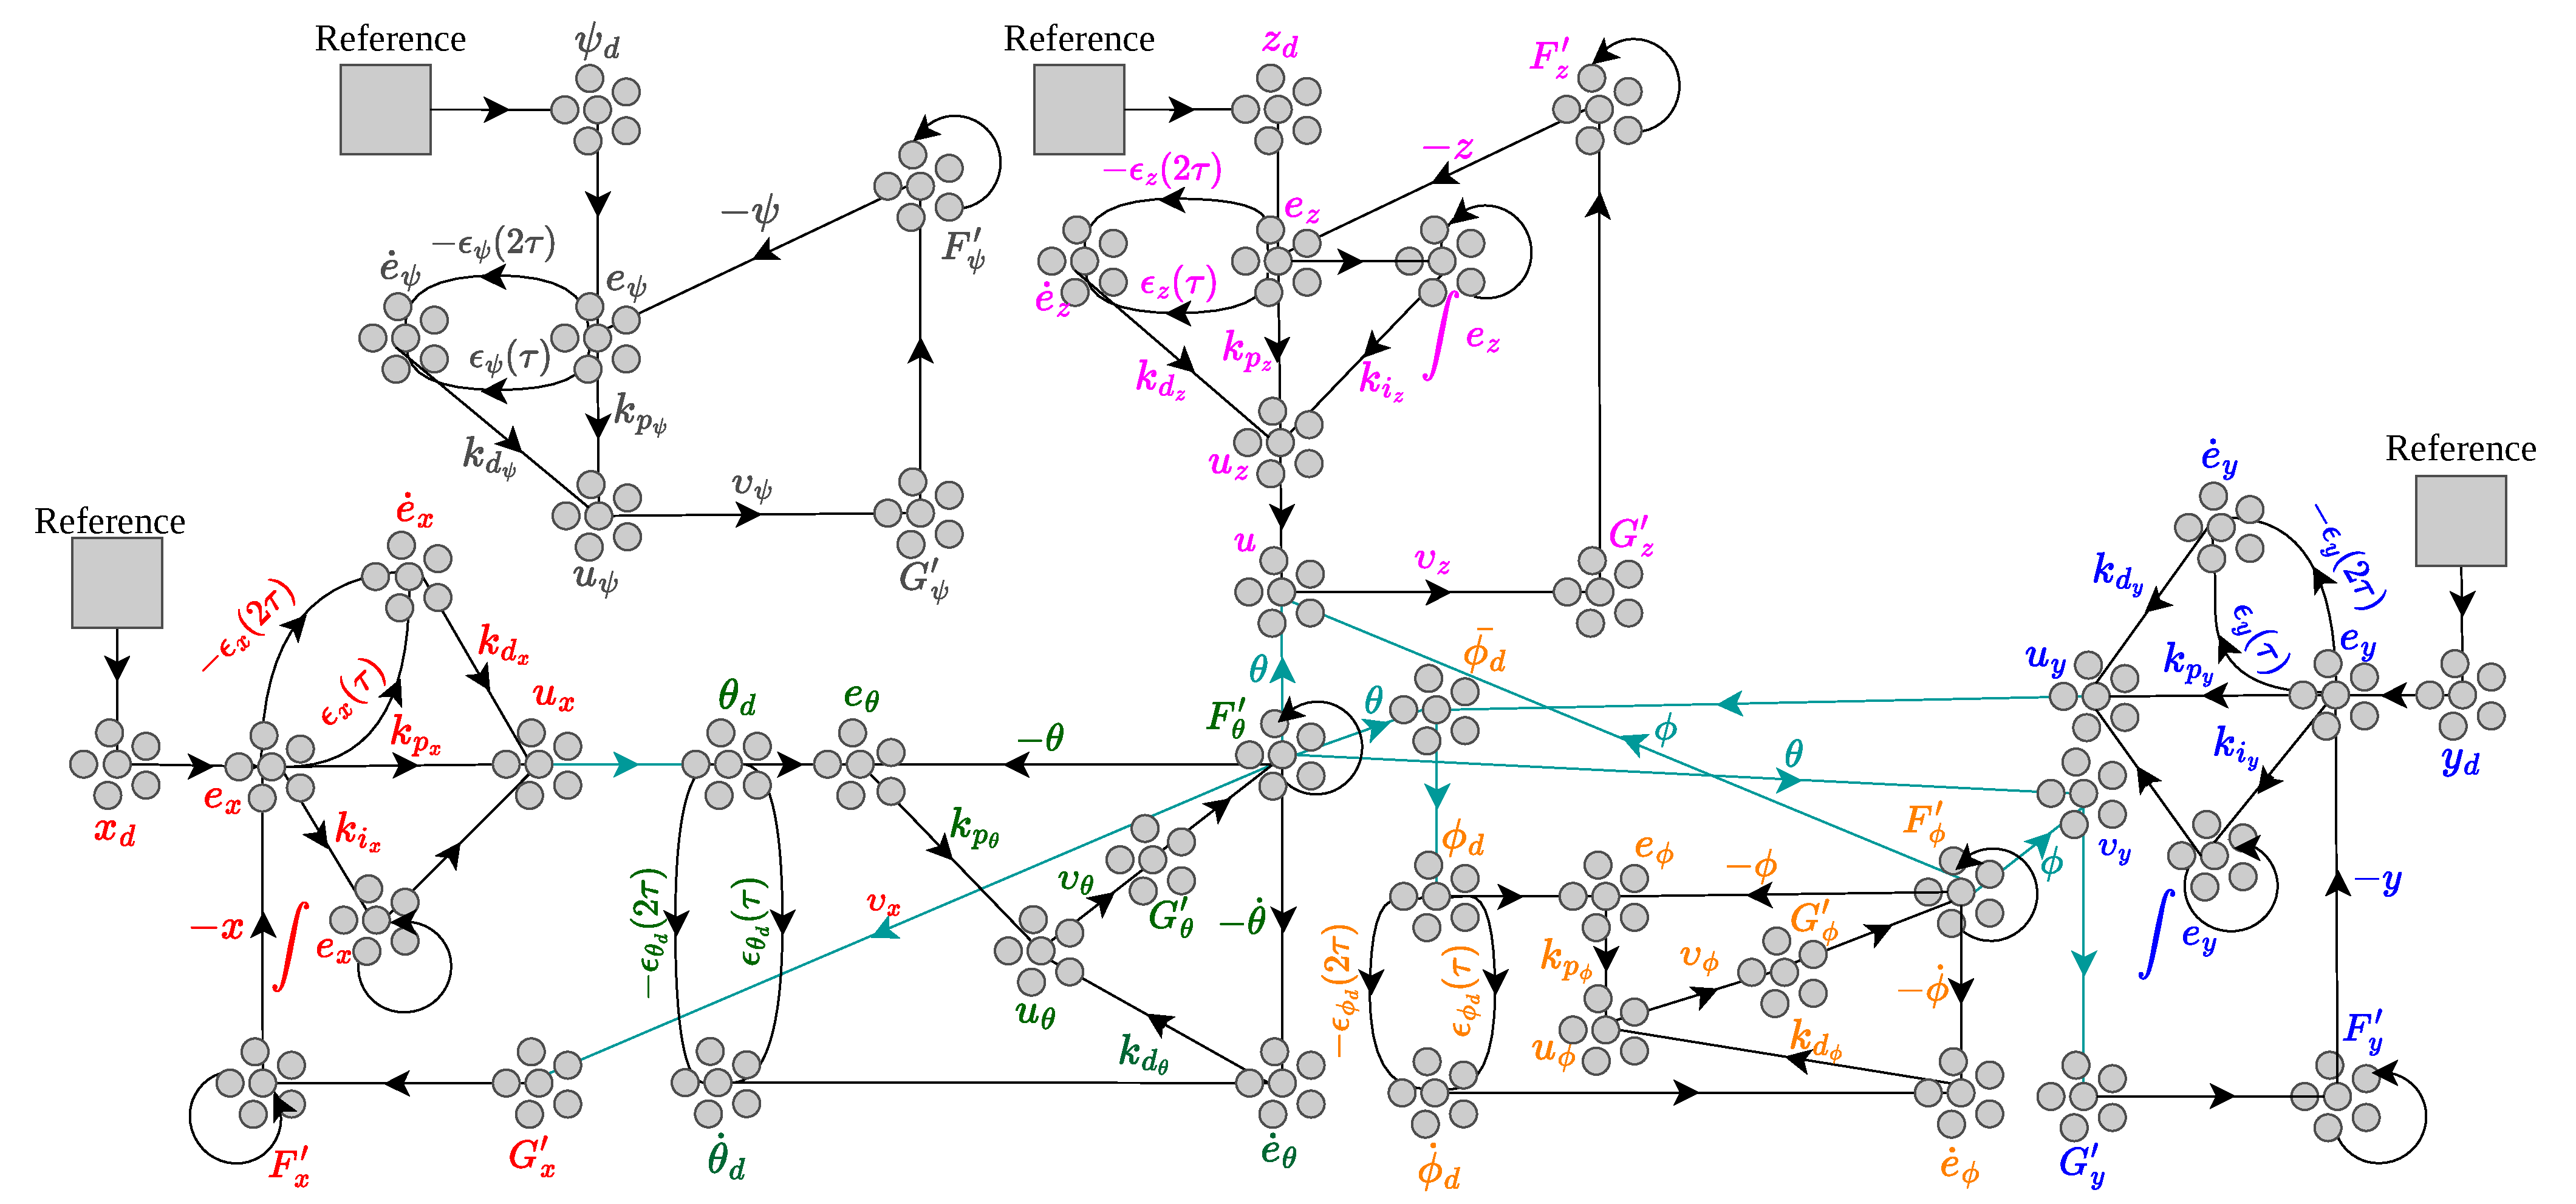
\includegraphics[width=\linewidth]{Figures/Digrama_UAV_dinamyc_ZXTheta-YPhi-3.pdf}
    \caption{The diagram is structured to show translation subsystems, as well as the orientations of the UAV, in a neural format. Each subsystem consists of interconnected neural networks that perform specific transformations for state-space representation and control law calculations. The flow of information is indicated by arrows, with cyan-colored arrows highlighting the dynamic couplings between the subsystems.}
    \label{fig:NengoGUI}
\end{figure*}
%
\noindent
where the integral gain $\mathbf{K}_i$ is incorporated into the input before the neural integration stage, following the approach proposed in~\cite{olivares_self-tuning_2026}. Consequently, the translational loops are implemented as neural PID controllers, whereas the rotational loops require only the proportional and derivative neural pathways.

\textbf{Algorithm}~\ref{Algoritmo-PID-classic} summarizes the neural implementation as a generic template for a subsystem $\zeta\in\{z,x,\theta,y,\phi,\psi\}$, following the unified state-space representation in~\eqref{eq:FG_generic}. The six control loops are obtained by instantiating this template with the corresponding state variables, control input, reference signal, and controller gains defined in Subsection~\ref{FG_subsystems}. The integral pathway is enabled only for the translational subsystems, yielding PID control, whereas the attitude subsystems implement PD control. The parameter ``dim'' specifies the dimensionality of the vector represented by each neural ensemble, ``transform'' defines the connection scaling matrix, ``radius'' determines the input range over which the NEF optimizes the decoding weights, and ``synapse'' denotes the synaptic filter time constant. The symbol ``$\rightarrow$'' represents a connection between ensembles or nodes. Finally, $T_{\mathrm{neu}}$ is the neural simulation time step, $n$ is the discrete-time index, and $t_f$ is the final simulation time.

% \begin{figure*}[!ht]
%     \centering
%     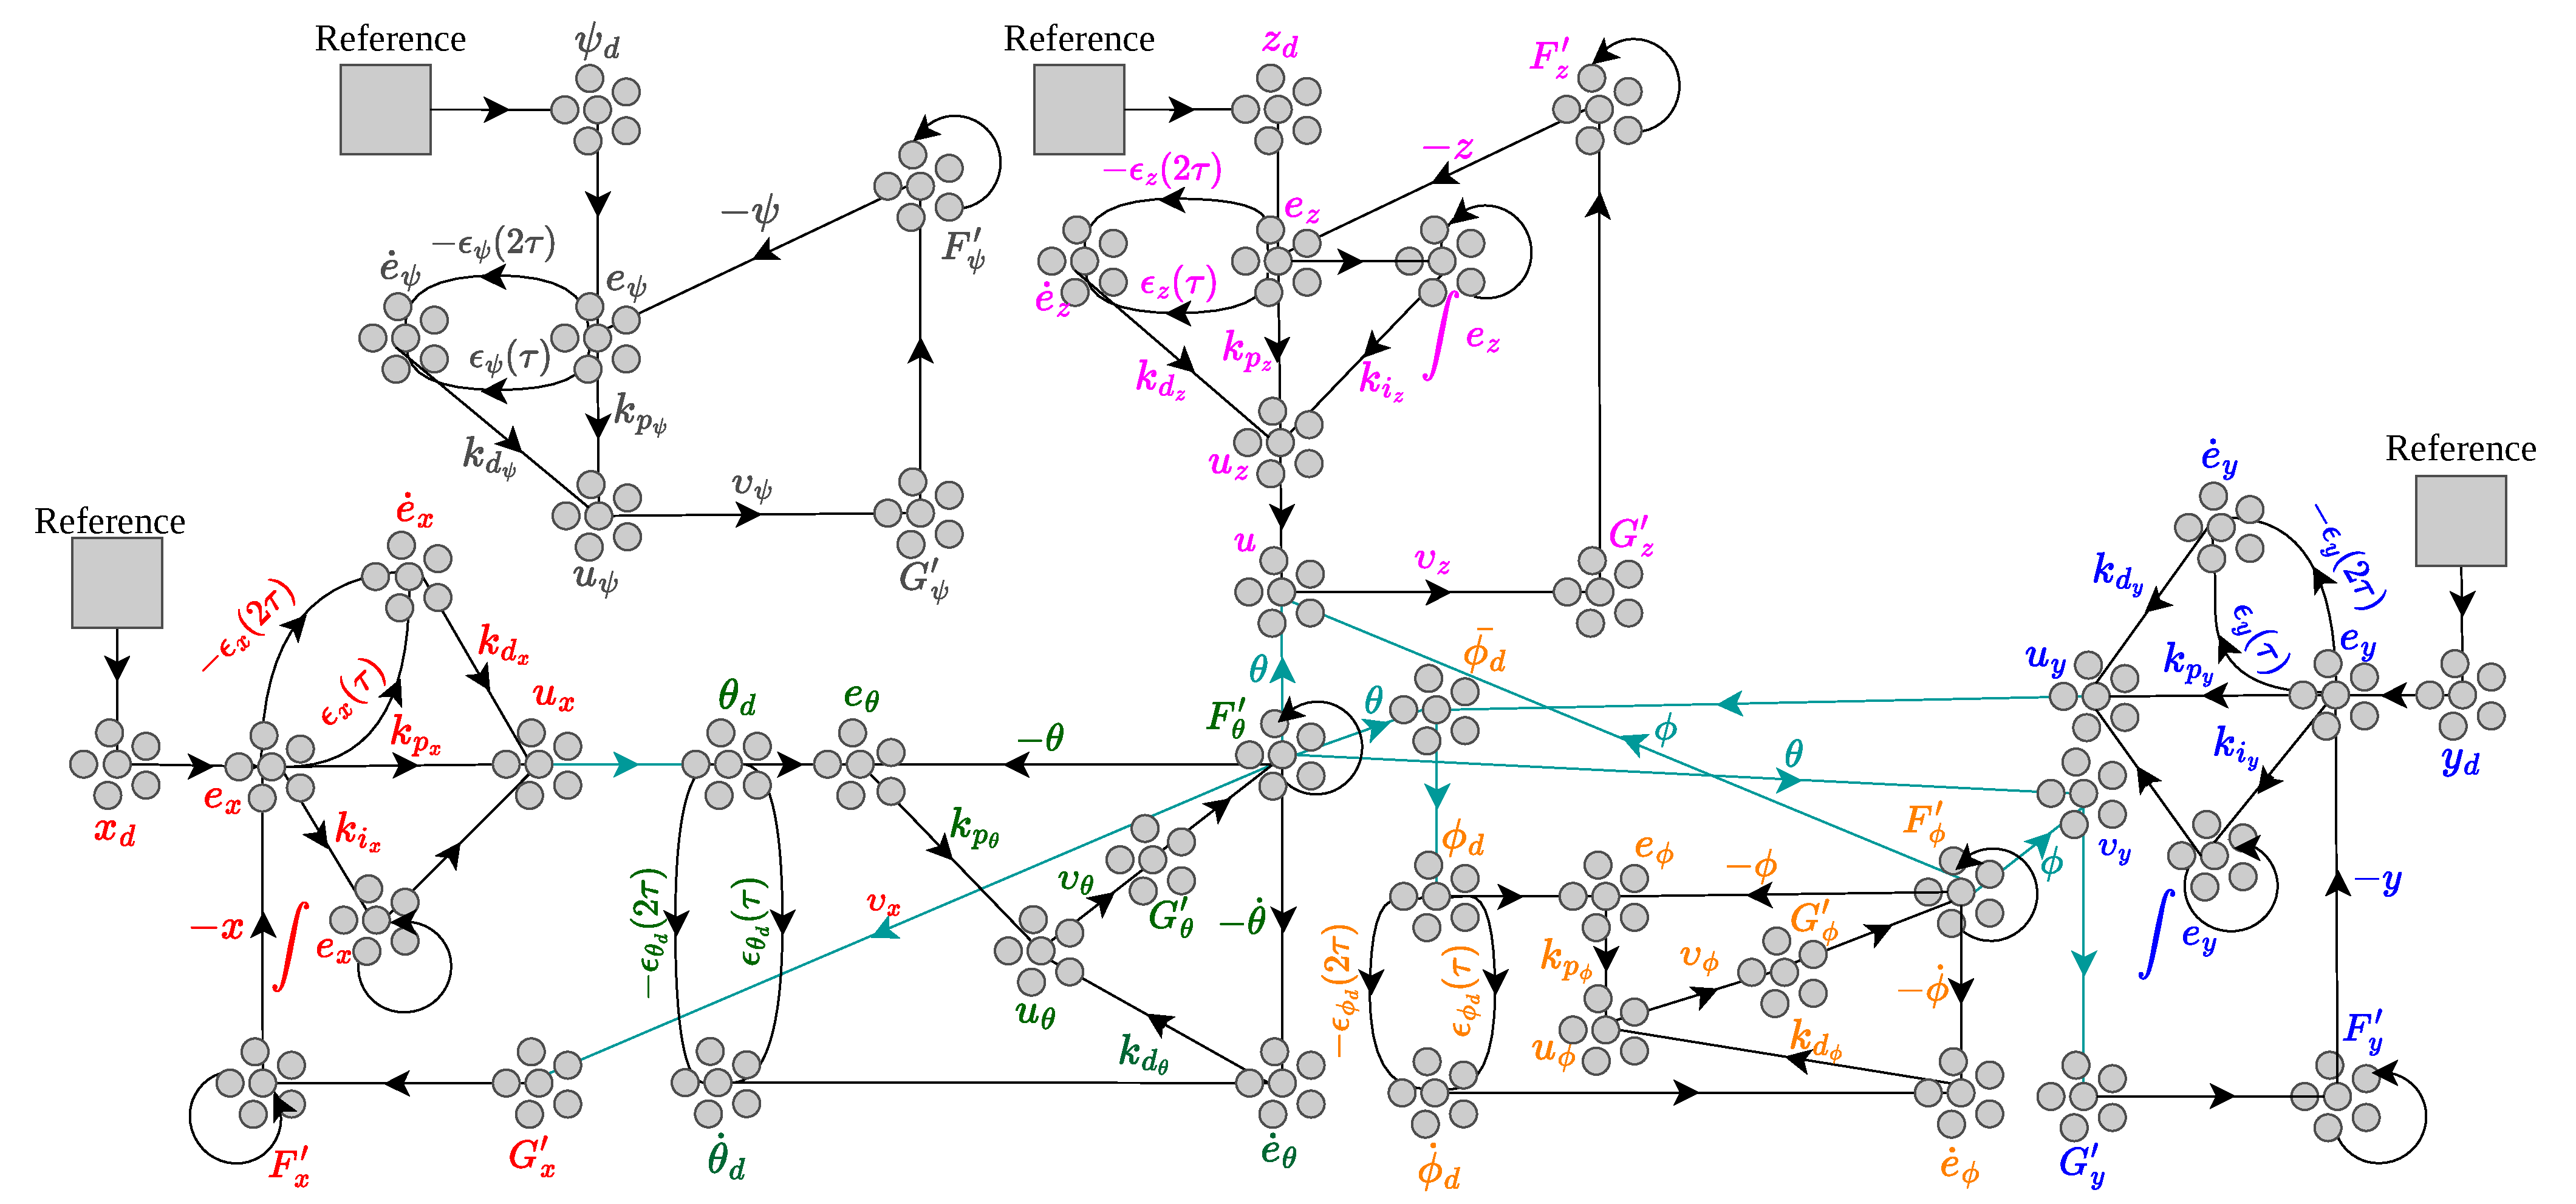
\includegraphics[width=0.97\linewidth]{Figures/Digrama_UAV_dinamyc_ZXTheta-YPhi-3.pdf}
%     \caption{The diagram is structured to show translation subsystems, as well as the orientations of the UAV, in a neural format. Each subsystem consists of interconnected neural networks that perform specific transformations for state-space representation and control law calculations. The flow of information is indicated by arrows, with cyan-colored arrows highlighting the dynamic couplings between the subsystems.}
%     \label{fig:NengoGUI}
% \end{figure*}

Fig.~\ref{fig:NengoGUI} visualizes the resulting neural flight-control architecture based on the reduced model of Section~\ref{Modeling}. Nengo's framework does not easily allow for complex nonlinear calculations within a single ensemble. Therefore, the diagram shows how elements like $u_y$ and $\theta$ are first combined in a shared ensemble (labeled $\bar{\phi}_d$) to perform operations such as $\phi_d = \tan^{-1}(u_y \cos\theta / g)$. Similarly, another ensemble (labeled $\upsilon_y$) is employed to facilitate calculations like $\upsilon_y = g \tan\phi / \cos\theta$, where the values of $\phi$ and $\theta$ are first brought together. This ensures that the nonlinear computations are represented within the spiking neural network.



\section{Simulation Results}\label{Simulations}
%
The performance of the proposed neuromorphic controller was evaluated against its conventional counterpart through numerical simulations conducted over a $60\,\mathrm{s}$ mission with a sampling period of $1\,\mathrm{ms}$. Both controllers executed the same 3D trajectory-tracking task under identical initial conditions and reference commands defined as:
%
\begin{equation}
\label{eq:mission}
\begin{aligned}
x_d(t) &= \frac{1}{1+e^{-(t-5)}}, \qquad
z_d(t) = \frac{-3}{1+e^{-(t-4)}},\\[2pt]
y_d(t) &=
\begin{cases}
0, & t < 15\,\mathrm{s},\\[2pt]
\dfrac{1.5}{1+e^{-(t-20)}}, & t \ge 15\,\mathrm{s},
\end{cases}, \qquad
\psi_d(t) = 0
\\[2pt]
%\psi_d(t) &= 0
% \begin{cases}
% \psi(0) &= 0.08~\mathrm{rad},\\[2pt]
% 0, & t > 0\,\mathrm{s}
% \end{cases}
\\[2pt]
\end{aligned}
\end{equation}

The mission begins with a vertical climb to an altitude of $3\,\mathrm{m}$ while simultaneously translating $1\,\mathrm{m}$ along the inertial $x_{\mathcal{I}}$ axis. After $15\,\mathrm{s}$, an additional lateral displacement of $1.5\,\mathrm{m}$ along the inertial $y_{\mathcal{I}}$ axis is commanded. The desired yaw angle is maintained at $\psi_d=0\,\mathrm{rad}$ throughout the maneuver. The vehicle is initialized from rest, with all translational and rotational states set to zero except for a small initial yaw offset of $\psi(0)=0.08\,\mathrm{rad}$.

%To ensure smooth motion and avoid abrupt control actions, the position references were generated using sigmoidal functions, yielding continuous trajectories with bounded velocities and accelerations. The reference trajectories are defined as
% The vertical channel is plotted as $-z$ (altitude) so that climbs read upward, consistent with the NED formulation of Section~\ref{Modeling}; the attitude channels are shown in the corresponding maneuver-positive sense.

\subsection{Simulink Simulation}

The control architecture described in Section~\ref{Control} was implemented in MATLAB/Simulink~R2025a with a fixed-step fourth-order Runge--Kutta integrator. %For this benchmark, the rotor-level allocation is replaced by the virtual total thrust and body-axis command inputs, so that the comparison focuses on the closed-loop controller and its neural realization. 
The cascaded baseline comprises outer position loops for $\theta_d$ and $\phi_d$ generation, inner attitude loops for $u_\theta$, $u_\phi$, and $u_\psi$, and the thrust law \eqref{eq:u}, as shown in Fig.~\ref{f:diagrama_control}. All gains and simulation parameters are listed in Table~\ref{tab:initParamPIDclassic}.
%
\begin{table}[h!]
\centering
\caption{Controller gains and simulation parameters (SNN/Nengo vs. classical MATLAB/Simulink).}
\label{tab:initParamPIDclassic}
\footnotesize
\setlength{\tabcolsep}{4.2pt}
\resizebox{\columnwidth}{!}{%
\begin{tabular}{llccc@{\hspace{9pt}}ccc}
\toprule
& & \multicolumn{3}{c}{SNN/Nengo} & \multicolumn{3}{c}{Classical MATLAB/Simulink} \\
\cmidrule(lr){3-5}\cmidrule(lr){6-8}
Controller & DOF controlled & $k_p$ & $k_d$ & $k_i$ & $k_p$ & $k_d$ & $k_i$ \\
\midrule
PID$_x$       & Position $x_\mathcal{I}$         & 8.8  & 0.1  & 0.3  & 1.6 & 5.0 & 0.08 \\
PID$_y$       & Position $y_\mathcal{I}$         & 10.3 & 4.2  & 0.7  & 3.0 & 2.0 & 0.10 \\
PID$_z$       & Position $z_\mathcal{I}$         & 40   & 5.0  & 0.1  & 40  & 5.0 & 2.00 \\
PD$_\theta$   & Attitude pitch $\theta$          & 90   & 12.1 & --   & 120 & 8.0 & -- \\
PD$_\phi$     & Attitude roll $\phi$             & 90   & 12.0 & --   & 40  & 8.0 & -- \\
PD$_\psi$     & Attitude yaw $\psi$              & 90   & 70   & --   & 7.0 & 4.0 & -- \\
\midrule
% \multicolumn{2}{l}{Simulation horizon} & \multicolumn{3}{c}{$60$~s} & \multicolumn{3}{c}{$60$~s} \\
% \multicolumn{2}{l}{Integration/simulation step} & \multicolumn{3}{c}{$1$~ms} & \multicolumn{3}{c}{$1$~ms} \\
\multicolumn{2}{l}{Integration method} & \multicolumn{3}{c}{NEF recurrent dynamics} & \multicolumn{3}{c}{fourth-order Runge--Kutta} \\
\multicolumn{2}{l}{Vehicle mass, $m$} & \multicolumn{3}{c}{$1$~kg} & \multicolumn{3}{c}{$1$~kg} \\
%\multicolumn{2}{l}{Gravity, $g$} & \multicolumn{3}{c}{$9.81$~m/s$^2$} & \multicolumn{3}{c}{$9.81$~m/s$^2$} \\
\multicolumn{2}{l}{Neurons per ensemble, $J$} & \multicolumn{3}{c}{200} & \multicolumn{3}{c}{--} \\
\multicolumn{2}{l}{Postsynaptic time constant, $\tau$} & \multicolumn{3}{c}{$0.1$~s} & \multicolumn{3}{c}{--} \\
%\multicolumn{2}{l}{General ensemble radius} & \multicolumn{3}{c}{5} & \multicolumn{3}{c}{--} \\
%\multicolumn{2}{l}{Integral-ensemble radius} & \multicolumn{3}{c}{1} & \multicolumn{3}{c}{--} \\
\bottomrule
\end{tabular}%
}
\end{table}


% The reference implementation of the control architecture of
% Section~\ref{Control} was developed in MATLAB/Simulink~R2025a at the subsystem
% level of Section~\ref{Modeling}. For this benchmark, the rotor-level allocation
% is replaced by the virtual total thrust and body-axis command inputs, so that
% the comparison focuses on the closed-loop controller and its neural realization. The cascaded baseline uses outer position loops to generate $\theta_d$ and $\phi_d$, inner attitude loops to command $\Gamma_\theta$, $\Gamma_\phi$, and $\Gamma_\psi$, and the thrust law \eqref{eq:u}. Simulink runs at $1$~kHz with fixed-step fourth-order Runge--Kutta integration; integral action is implemented as a discrete accumulator with anti-windup (Fig.~\ref{f:diagrama_control}). All gains and simulation settings are reported in Table~\ref{tab:initParamPIDclassic}.

% In this benchmark ($m=1$~kg), the classical controller achieves position RMSEs of $0.008$~m, $0.013$~m, and $0.019$~m on the $x_\mathcal{I}$, $y_\mathcal{I}$, and $z_\mathcal{I}$ axes, respectively, with no actuator saturation (thrust within $[9.1,\,12.0]$~N and commanded tilt below $0.7^{\circ}$). This response provides the ground truth for the neuromorphic comparison.

\subsection{Nengo Simulation}

The SNN gains were adjusted through a heuristic procedure based on observation of the system's performance, which yielded the values for the gains $\textbf{K}_p$, $\textbf{K}_i$, and $\textbf{K}_d$, as well as the number of neurons and the postsynaptic time constant. These values, presented in Table~\ref{tab:initParamPIDclassic}, are used throughout the neuromorphic implementation.



Fig.~\ref{fig:sim_states} compares the translational and attitude responses of the SNN-based controller with the classical MATLAB/Simulink implementation and the reference trajectories. Both controllers exhibit similar trajectory-tracking performance, with the neural controller achieving high agreement with classical counterpart across all degrees of freedom. 
%
\begin{figure}[h!]
\centering
\includegraphics[width=\columnwidth]{Comrob_Hexa2026/Figures_2/fig01_states_v5_rad.pdf}
\caption{Closed-loop states: translational positions (left) and attitude angles (right). Reference: (\legdotted{black}) dotted black; classical MATLAB/Simulink: (\legsolid{matlabBlue}) solid blue; SNN/Nengo: (\legsolid{red}) solid red. %The vertical position is shown as $-z$ (altitude), consistent with the NED formulation of Section~\ref{Modeling}; yaw is regulated at $\psi_d=0$.
}
\label{fig:sim_states}
\end{figure}

Fig.~\ref{fig:sim_commands} presents the corresponding control commands $u$, $u_\phi$, $u_\theta$, and $u_\psi$, where the neuromorphic and classical controllers produce silimar outputs. 
%
\begin{figure}[!t]
\centering
\includegraphics[width=\columnwidth]{Comrob_Hexa2026/Figures_2/fig02_commands_v5_rads2.pdf}
\caption{Control commands. Total thrust $u$ and virtual translational commands $u_x$ and $u_y$ (left), and normalized attitude commands $u_\psi$, $u_\theta$, and $u_\phi$ (right). Classical MATLAB/Simulink: (\legsolid{matlabBlue}) solid blue; SNN/Nengo: (\legsolid{red}) solid red.}
\label{fig:sim_commands}
\end{figure}



The quantitative performance comparison is summarized in Table~\ref{tab:benchmark}.
%

% \begin{table}[h!]

% \caption{Tracking performance over the $60$~s mission: RMSE, maximum absolute error, steady-state error (SSE), and SNN--classical correlation ($\rho_{\mathrm{SNN,cls}}$).}
% \label{tab:benchmark}
% \centering
% \footnotesize
% \setlength{\tabcolsep}{4.5pt}
% \begin{tabular}{lcccccc}
% \toprule
%  & \multicolumn{2}{c}{RMSE} & \multicolumn{2}{c}{ISE} & \multicolumn{2}{c}{SSE}\\
% \cmidrule(lr){2-3}\cmidrule(lr){4-5}\cmidrule(lr){6-7}
% Variable & Classical & SNN & Classical & SNN & Classical & SNN \\
% \midrule
% $x$ [m]        & $0.008$ & $0.032$ & $3.95 \times 10^{-3}$ & $0.0627$ & $0.000$ & $-0.031$\\
% $y$ [m]        & $0.013$ & $0.033$ & $0.0101$ & $0.0660$ & $0.000$ & $0.029$\\
% $z$ [m]       & $0.019$ & $0.048$ & $0.0213$ & $0.1367$ & $-0.001$ & $0.027$\\
% $\theta$ [rad] & $0.000$ & $0.005$ & $6.38 \times 10^{-6}$ & $1 . 71 \times 10^{-3}$ & $0.000$ & $-0.001$\\
% $\phi$ [rad]   & $0.001$ & $0.012$ & $5.68 \times 10^{-5}$ & $8 . 67 \times 10^{-3}$ & $0.000$ & $-0.004$\\
% $\psi$ [rad]   & $0.007$ & $0.009$ & $2.63 \times 10^{-3}$ & $4 . 61 \times 10^{-3}$ & $0.000$ & $0.002$\\
% \midrule
% \multicolumn{7}{l}{$\rho_{\mathrm{SNN,cls}}$:\; $x$: $0.9993$;\quad
% $y$: $0.9998$;\quad $-z$: $0.9992$}\\
% \bottomrule
% \end{tabular}
% \end{table}






%Both controllers accomplish the maneuver with sub-decimeter tracking error. The SNN-based implementation closely matches the classical baseline in both states (Fig.~\ref{fig:sim_states}) and commands (Fig.~\ref{fig:sim_commands}), with translational correlations $\rho_{\mathrm{SNN,cls}}\ge 0.999$ and position RMSEs below $5$~cm (Table~\ref{tab:benchmark}). The remaining differences are consistent with finite-population NEF decoding effects: (i)~a high-frequency spiking component on decoded signals; (ii)~small steady-state offsets (SSE on the order of $\pm 3$~cm in position and $\pm 0.004$~rad in attitude) and constant attitude biases (visible in Fig.~\ref{fig:sim_states}); and (iii)~a short initialization transient while neural states converge. This near-equivalent closed-loop behavior is obtained with a fully spiking controller using $J=200$ neurons per ensemble, supporting direct deployment on neuromorphic processors~\cite{dewolf_neuromorphic_2023,rajendran_low-power_2019}.
The comparison between the two control strategies was conducted using two error performance indices: Root Mean Square Error (RMSE) and Integral of Squared Error (ISE). Furthermore, the correlation coefficient $\rho_{\mathrm{SNN,cls}}$ was computed to quantify the similarity between the SNN-based and classical controller signals. As detailed in Table~\ref{tab:benchmark}, the low RMSE, ISE values and correlation coefficients exceeding $0.9$ confirm that the neuromorphic implementation achieves similar performance to the classical baseline, in terms of state trajectories (Fig.~\ref{fig:sim_states}). The discrepancies that remain are consistent with limitations of the NEF, including decoding errors arising from finite neural ensembles and the inherent differences in activation functions between leaky integrate-and-fire (LIF) neurons and rectified linear neurons. Specifically, the representational power of spiking neurons is bounded by their maximum firing rates, which can lead to saturation effects under large input amplitudes~\cite{dewolf_neuromorphic_2023,rajendran_low-power_2019}.

\begin{table}[h!]

\caption{Tracking performance over the $60$~s mission: RMSE, ISE, and SNN--classical correlation ($\rho_{\mathrm{SNN,cls}}$).}
\label{tab:benchmark}
\centering
\footnotesize
\setlength{\tabcolsep}{4.5pt}
\begin{tabular}{lcccc}
\toprule
 & \multicolumn{2}{c}{RMSE} & \multicolumn{2}{c}{ISE} \\
\cmidrule(lr){2-3}\cmidrule(lr){4-5}
Variable & Classical & SNN & Classical & SNN \\
\midrule
$x$ [m]        & $0.008$ & $0.032$ & $3.95 \times 10^{-3}$ & $0.0627$ \\
$y$ [m]        & $0.013$ & $0.033$ & $0.0101$ & $0.0660$ \\
$z$ [m]       & $0.019$ & $0.048$ & $0.0213$ & $0.1367$ \\
$\theta$ [rad] & $3 . 26 \times 10^{-4}$ & $0.005$ & $6.38 \times 10^{-6}$ & $1 . 71 \times 10^{-3}$ \\
$\phi$ [rad]   & $9 . 73 \times 10^ {-4}$ & $0.012$ & $5.68 \times 10^{-5}$ & $8 . 67 \times 10^{-3}$ \\
$\psi$ [rad]   & $6 . 62 \times 10 ^{-3}$ & $0.009$ & $2.63 \times 10^{-3}$ & $4 . 61 \times 10^{-3}$ \\
\midrule
\multicolumn{5}{l}{$\rho_{\mathrm{SNN,cls}}$:\; $x$: $0.9993$;\quad
$y$: $0.9998$;\quad $-z$: $0.9992$}\\
\bottomrule
\end{tabular}
\end{table}

\section{Conclusions and future work}\label{Conclusions}
This paper presented a neuromorphic modeling and control framework for a coaxial hexarotor UAV, where the reduced nonlinear vehicle dynamics and a cascaded flight-control architecture were implemented as spiking neural networks using the Neural Engineering Framework in the Nengo simulator. The proposed controller was evaluated in a 60 s trajectory-tracking mission and compared with a conventional cascade controller.

The results demonstrate that the SNN-based controller closely matches the performance of its conventional counterpart, achieving correlation coefficients above 0.99 and low RMSE and ISE values in translational trajectory tracking. These findings confirm that NEF-based SNNs can accurately reproduce classical flight-control behavior while maintaining closed-loop performance.

The proposed framework provides a modular and scalable approach for implementing UAV dynamics and flight-control algorithms as interconnected spiking neural populations, establishing a foundation for integrating more advanced, robust, adaptive, and learning-based neuromorphic controllers.

Future work will extend the framework to the complete nonlinear UAV model, including rotor and actuator dynamics, evaluate robustness under disturbances and uncertainties, and deploy the controller on dedicated neuromorphic hardware for real-time flight experiments.


\bibliographystyle{IEEEtran}
\bibliography{references}





\end{document}
